% !TEX encoding = UTF-8 Unicode
% !TEX root = ../Rapport/rapport.tex

\section{Branch and bound}

\subsection{Principe général du branch\&bound}
La méthode de Branch and Bound est une méthode arborescente exacte resposant sur un principe très
simple : lors de la résolution d'un problème toutes les solutions réalisables ne sont pas
intéressantes. Cette méthode cherche donc à réduire au maximum l'espace des solutions réalisables.

Pour ce faire, elle supprime une des contraintes du problème afin de se ramener à un problème
polynomial dont la solution est une borne inférieure du problème initial. Elle examine alors la
solution deux cas se présentent alors : \begin{enumerate}
	\item la solution est une solution réalisable, cette dernière est alors sauvegardée et sera
		utilisée utltérieurement
	\item la solution n'est pas réalisable, l'algorithem rajoute alors au problème considéré des
		contraintes de façon à se rapprocher d'une solution réalisable. Il s'agit d'une opération de
		branchement\footnote{On parle aussi de séparation.}.
\end{enumerate}

Prenons par exemple le problème du voyageur de commerce étudié plus loin, nous ramenons ce problème
à la recherche d'un arbre couvrant de poids minimum. Dans ce cas c'est la contrainte protant sur les
degrés des sommets qui est relaxée\footnote{On peut aussi relaxer la contrainte de connexité du
cycle qui nous ramènerait alors à un problème de couplage parfait de poids minimum.}. Il paraît
peu probable d'obtenir par cette relaxation une solution réalisable du TSP, alors une fois l'ACPM
obtenu, un sommet violant la contrainte relaxée est choisi et l'opération de branchement consiste en
la création de nouveaux problèmes, tous identiques au problème relaxé à un détail près : pour chaque
instance, on interdit une des arêtes adjacentes au sommet de dégré supérieur à 2 afin de forcer,
petit à petit, la non violation de cette contrainte et donc de se rapprocher d'une solution
réalisable. Dans le cas du TSP, la méthode de Branch and Bound, crée autant de nouveaux problèmes
que d'arêtes adjacentes au sommet choisi.

Présenté ainsi, la méthode branch and bound ne présente aucun intérêt par rapport à l'énumération de
l'ensemble des solutions, bien au contraire, son exécution est beaucoup plus lente que ce dernier.
Seulement, cette méthode garde en mémoire, la mémoire solution réalisable trouvée. Elle n'explorera
alors que les n\oe uds de l'arbre créé dont la borne est inférieure à la solution réalisable
sauvegardée \footnote{On explorera les n\oe uds dont la borne est supérieure à la solution
réalisable dans le cas d'une problème de maximisation.}. En effet, à chaque itération de
l'algorithme la solution du problème relaxé est une borne inférieure de toute solution réalisable
vérifiant les contraintes imposées par l'algorithme, donc rajouter de nouvelles contraintes
augmenterait la valeur des futures solutions. Possédant une solution meilleure que cette borne, il
serait stupide de s'obstiner à explorer ces branches. 

Cette opération, appelée élagage de l'arbre, permet de réduire considérablement le nombre de n\oe ds
de ce dernier et donc le nombre de calculs.

\subsection{Méthode de séparation}
Comme vu précédemment, il s'agit de la méthode permettant la création de nouveaux problèmes soumis à
des conditions plus strictes que celles auxquelles est soumise le problème parent.

Dans le cadre des nos travaux, nous avons utilisé les arbres couvrants de poids minimimaux. La
séparation consiste alors en la sélection d'un n\oe ud de degré 3 au plus de l'ACPM et en
l'interdiction de chacune des arêtes.

\subsection{Méthode d'évaluation}
La méthode d'évaluation désigne le problème relaxé utilisé pour trouver rapidement une borne du
problème initial. Ici nous avons utilisé la recherche d'un ACPM sur le graphe initial auquel nous
avons retiré arbitrairement un sommet. Une fois l'ACPM calculé, le sommet retiré est ajouté à
ce dernier par l'intermédiaire de ces deux arêtes adjacentes de poids le plus faible.

Une solution réalisable est alors trouvée lorsque l'ACPM retourné est une chaîne, dont chaque
extrêmité est adjacente à l'une des deux arêtes de poids le plus faible sortant du sommet retiré.


\subsection{Stratégie de parcours}
La stratégie de parcours définit dans quel ordre seront exploré les n\oe uds de l'arbre généré. En
règle général, la stratégie de recherche en profondeur sera utilisée, puisqu'elle permet de mettre à
jour rapidement la meilleure solution réalisable sauvegardée par l'algorithme.


\subsection{Solution initiale du voyageur de commerce}

Un point important de l'algorithme de Branch and Bound est le calcul initial d'une solution
réalisable qui servira de borne. Le but étant d'obtenir une borne le plus proche possible de la
solution optimale, ce qui permettra d'élaguer très rapidement l'arbre, et ce en un temps
raisonnable.

Dans le cadre de ces travaux, nous avons utilisés la chaîne de poids le plus faible complétée par
une arête pour obtenir un cycle hamiltonien. 

Les résultats des temps d'exécution sont présentés à la figure \ref{tsp_chaine}. On remarquera la forme
exponentielle de la courbe de résultats.

D'autres stratégies peuvent être choisies comme point de départ, on peut par exemple citer 2-opt
permettant l'amélioration d'un cycle en analysant les 2-permutations de celui-ci : si en échangeant
les extrêmités de deux arêtes on améliore le cycle alors, on réalise la permutation.

\begin{figure}[H]
	\begin{center}
	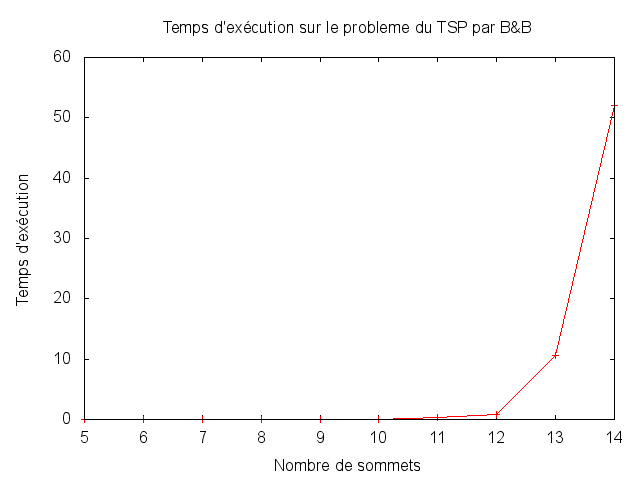
\includegraphics[width=\linewidth]{../pratique/branch_and_bound_dev/tsp_bb.png}
\end{center}
\caption{Représentation graphique du temps d'exécution de l'algorithme de Branch and Bound en
fonction du nombre de villes à visiter}
\label{tsp_chaine}
\end{figure}

\subsection{Comparaisons}

\begin{figure}[H]
	\begin{center}
	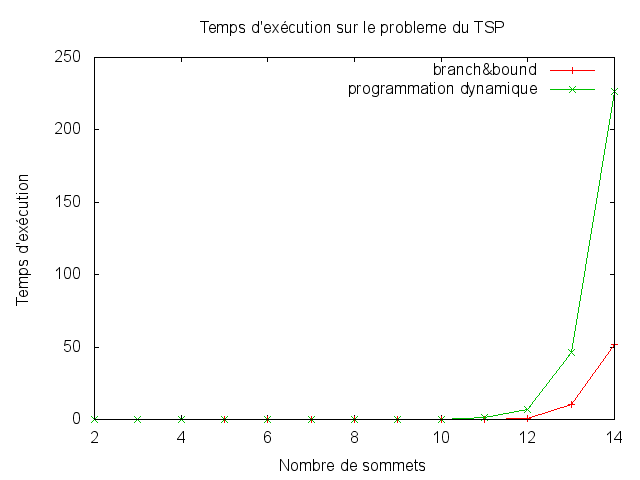
\includegraphics[width=\linewidth]{../pratique/comp.png}
\end{center}
\caption{Comparaison du temps d'exécution des algorithmes Branch and Bound et de programmation
dynamique en fonction du nombre de sommets}
\label{comp_algo}
\end{figure}

La figure \ref{comp_algo} met en avant le temps gagné (en moyenne) par des algorithmes de branch and
bound. On observe que pour des problèmes mettant en scène 14 villes, le Branch and Bound présente un
temps d'exécution moyen plus de quatre fois inférieur au temps d'exécution de la programmation
dynamique. 

Ceci met en avant le nombre très important d'opérations économisées par l'élagation de l'arbre. En
effet, il ne faut pas oublier qu'à chaque étape de l'algorithme de branch and bound, ce dernier
résouds un problème relaxé ce qui représente là un nombre considérable d'opérations et malgré ceci
le branch and bound est beaucoup plus rapide.

On confirme alors que le nombre de solutions réalisables intéressantes et très faible par rapport à
la taille de l'espace des solutions.

\section{Conclusion}

Malheureusement, nous n'avons pas pu mettre en \oe uvre d'autres algorithmes d'initialisation pour
le branch and bound du TSP, ce qui aurait permis de mettre en avant l'importance de la solution
acceptable initiale sur le temps d'exécution de l'algorithme.

Théoriquement parlant, plus la solution initiale est proche de la solution optimale, plus le temps
d'exécution est faible. Seulement, réduire la marge d'erreur lors de l'initialisation implique un
calcul plus long. Il faut donc trouver le juste équilibre entre le temps consacré à l'initialisation
et celui consacré à la résolution.

Il aurait été intéressant de pouvoir mettre en \oe uvre l'algorithme de Christophides afin de
pouvoir comparer les résultats en temps et en précision de tous ces algorithmes.
